\subsection{ANTELOPE (Semi-supervised)}
\label{subsec:unsupervised}

The semi-supervised analysis approach broadens the discovery sensitivity of the search through the use of semi-supervised ML, where training of the model is data-driven and labels are only partially provided during training.
While broad sensitivity is a general key goal of LHC searches, it is particularly motivated in the case of dark QCD models, which can lead to widely varying topologies depending on the values of model parameters.
In the case of SVJs, the \rinv~fraction in the jet can dramatically vary the \met, shower shape, and other key features, making it difficult to find a single standard analysis variable that can distinguish all signal topologies from QCD.

%--------------------
\subsubsection{Architecture Fundamentals}
The model-independent search region of this analysis is implemented with a novel ML approach that builds on the ANTELOPE architecture to construct a tool that is capable of performing low-level anomaly detection with permutation-invariant inputs.
This tool, referred to as \textbf{ANomaly deTEction on particLe flOw latent sPacE (ANTELOPE)}, is a custom solution designed for this analysis.

ANTELOPE uses the supervised signal vs. background training of the PFN network described in the previous section to generate a permutation invariant latent space that is representative of the original input variables, encodes the input events into these latent space variables $\mathcal{O}$, and trains a \textit{variational autoencoder} (VAE) over the events modeled as PFN latent space variables. A VAE is a common architecture used for anomaly detection and data-driven ML training. It has been used in previous ATLAS searched to model jet level information, such as the search presented in \cite{yxh} using the recurrent architecture described in \cite{vrnn}. One of the limitations of a recurrent architecture is the need to order the low level inputs, which affects the performance of the tool. Jet constituent information is intrinsically unordered, and therefore a permutation invariant approach removes this element of arbitrary decision making from the modeling process. A visual example of the ANTELOPE inputs is given in Figure~\ref{fig:antelope_input_rep}. 

\begin{figure}[!htbp]
\centering
   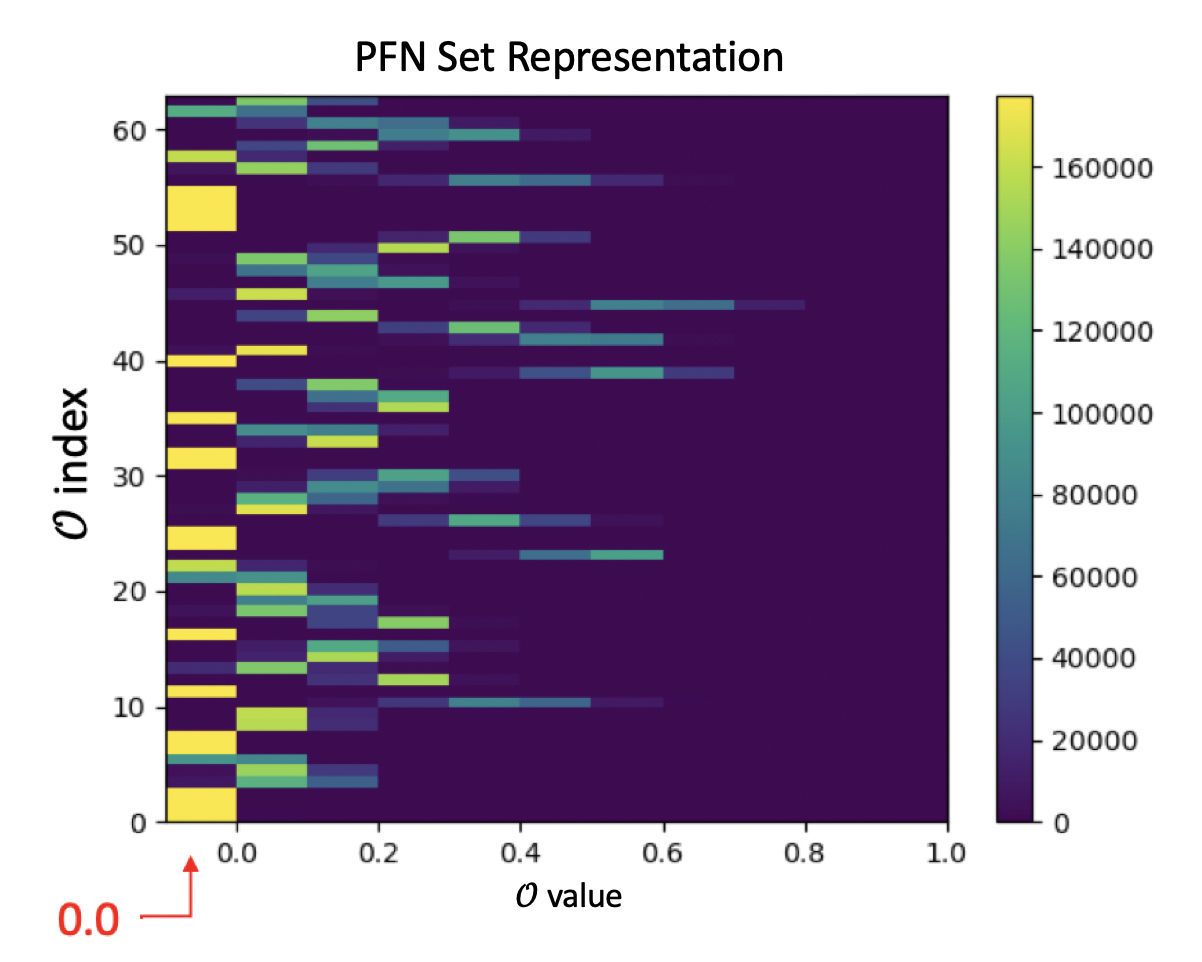
\includegraphics[width=0.9\textwidth]{figures/ml/antelope_input_rep}
    \caption{A visual representation of the 64 PFN latent space variables which create the input of the VAE component of ANTELOPE. The left shows a 2D histogram of the PFN latent space index (0-63) versus the value assumed by that index. The right shows 1D histograms of two particular PFN latent space variables. 
    \label{fig:antelope_input_rep}}
\end{figure}

The input to the model is the same 6 track variables for the leading 160 tracks of the leading two jets, as presented in Section~\ref{sec:input_model}. The track information is encoded to the PFN $\Phi$ latent space using the pre-trained $\Phi$ network (trained according to the steps outline in Section~\ref{sec:pfn_training}. The resulting $\Phi$ basis is summed to created the fixed length symmetric representation $\mathcal{O}$. The VAE is then trained in an unsupervised way using inputs encoded to $\mathcal{O}$ from data events only. The VAE is given no knowledge of the signal model during training. 
It is able to perform anomaly detection through an encoder stage which does a lossy compression on the input to a lower-dimensional latent space, and a decoder stage that samples from that latent space and generates an output of the original dimensionality.
By using the reconstruction error as a loss, this process enables the VAE to develop a knowledge of the underlying data structure, thereby isolating new out-of-distribution events by their high reconstruction error. 
This strategy is semi-supervised because the tool has some knowledge of correct labels (eg. through the PFN latent space embedding) but is followed by a data-driven unsupervised stage. 

Figure~\ref{fig:antelope_arch} provides a diagram of the ANTELOPE architecture.
\begin{figure}[!htbp]
\centering
   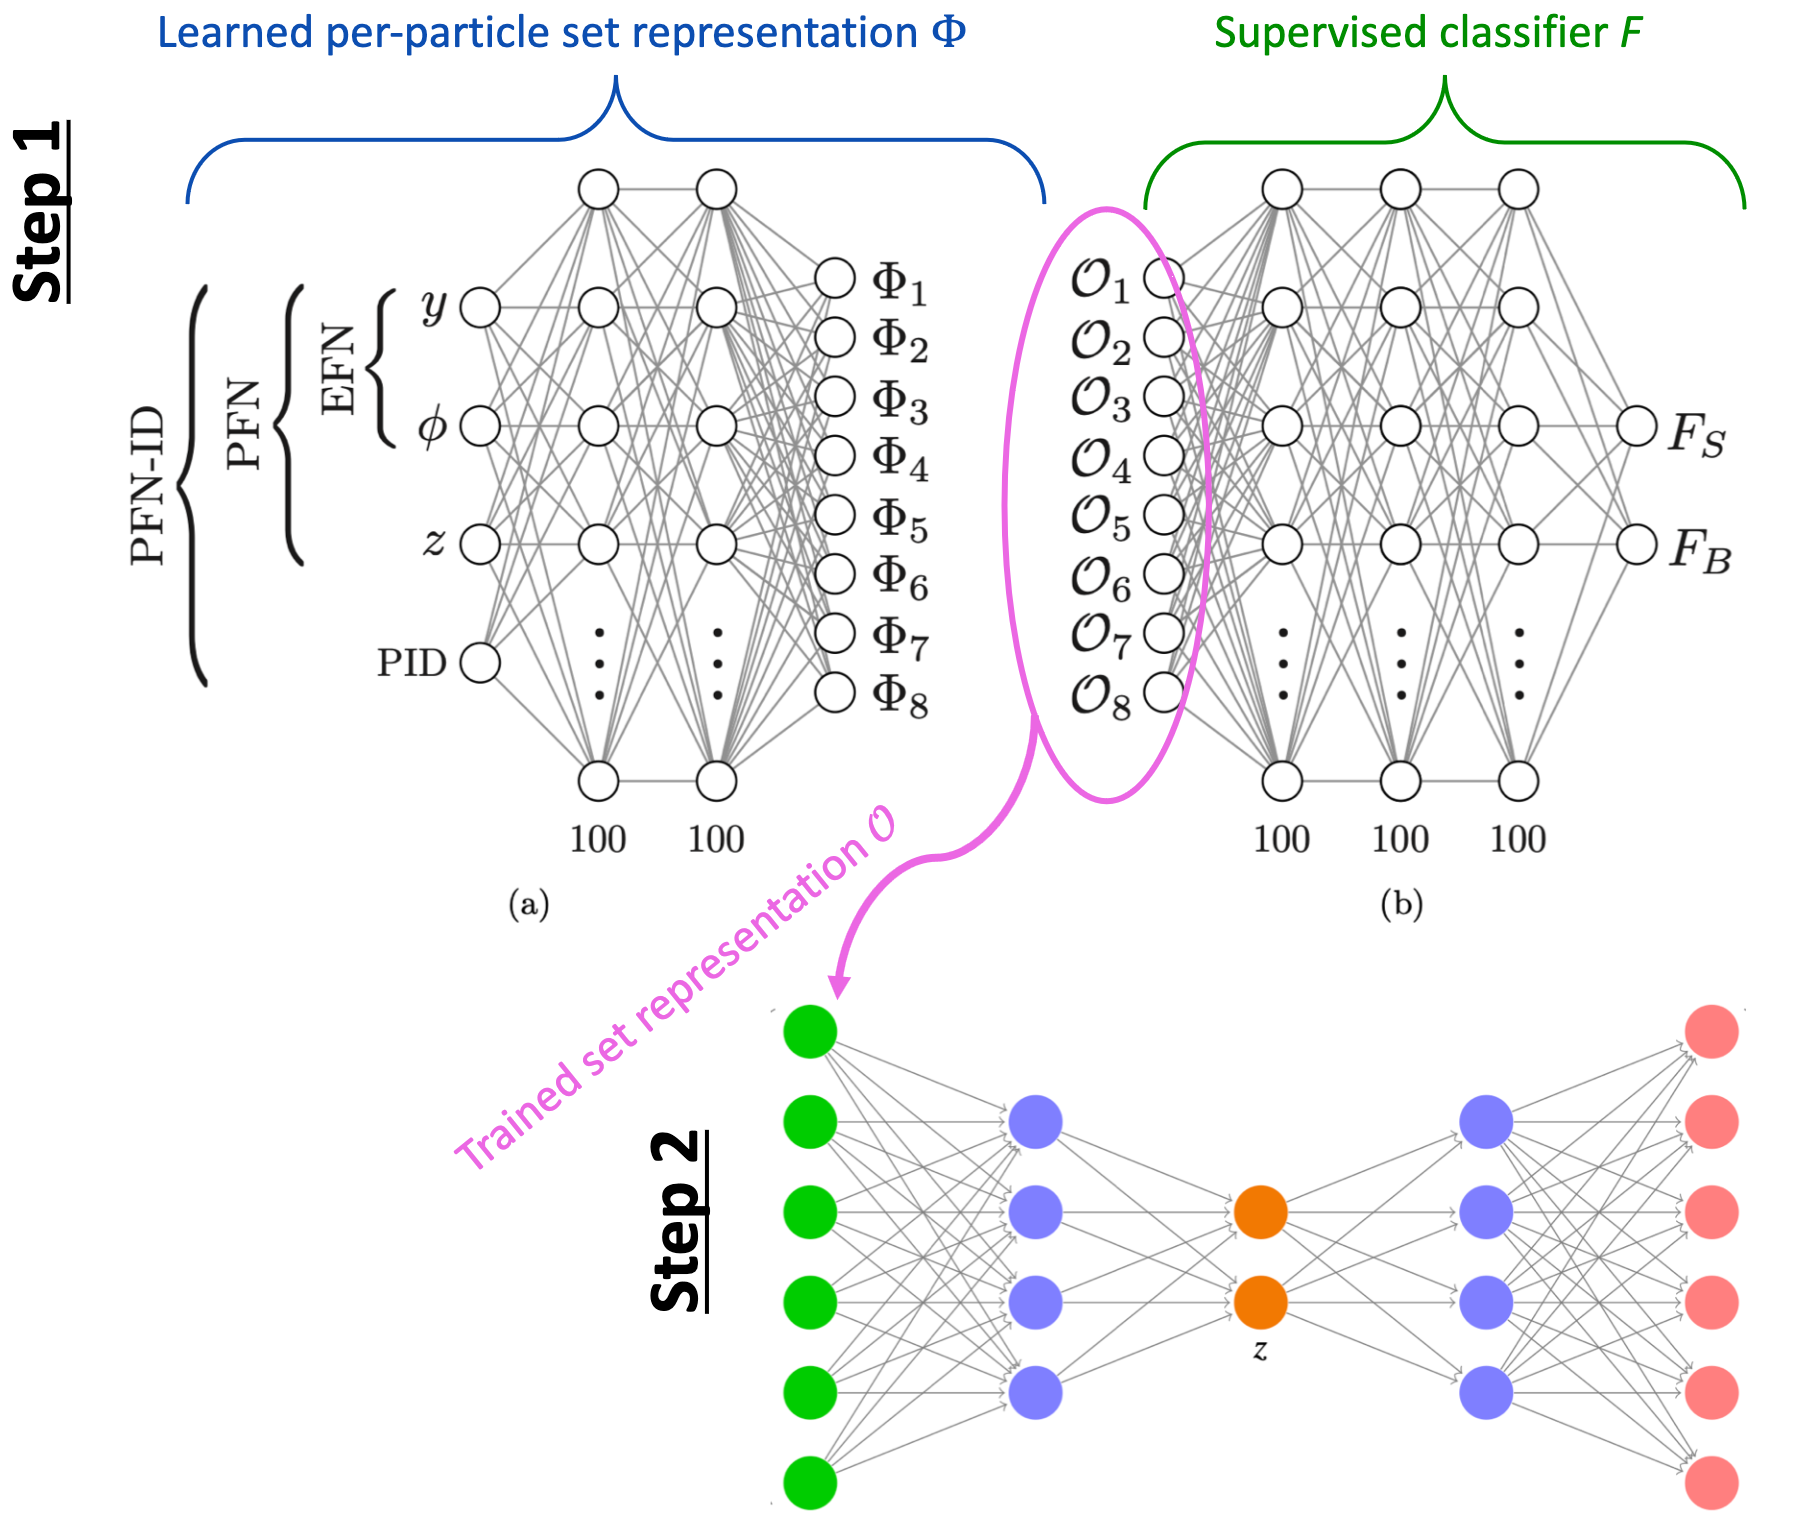
\includegraphics[width=0.9\textwidth]{figures/ml/antelope_arch}
    \caption{An annotated diagram of the ANTELOPE architecture.
    \label{fig:antelope_arch}}
\end{figure}


%--------------------
\subsubsection{Training}

The VAE stage of the ANTELOPE network is trained directly over a subset of data events at preselection (6.7 million available, 500,000 used, with a 80\% / 20\% training/test split).
The input dimensionality of the VAE has to match the encoded $\Phi$ dimension of the PFN, in this case 64. 
The encoder has an encoding layer that brings the dimensionality to 32, and a final layer that compresses to the latent space dimension of 12. 
The network is trained for 50 epochs, with a learning rate of 0.00001.  
The loss $\mathcal{L}$ is the sum of two terms, the mean-squared error (MSE) of input-output reconstruction, and the Kullback-Leibler divergence (KLD).

\begin{equation}
\label{eq:vrnnloss}
\mathcal{L} = \sum_i L_i = \sum_i | \Phi_i^2 - \Phi\prime_i |^2 + \lambda D_{\text{KL}}
\end{equation}

As the PFN inputs are sufficiently normalized to remove any spurious information from training, no additional normalization is applied to the PFN encoded inputs.
The final ANTELOPE score used in the analysis is produced by applying a log + sigmoid transformation function to the total evaluated loss $\mathcal{L}$. 

Figure~\ref{fig:antelope_loss} shows the loss during training.
\begin{figure}[!htbp]
\centering
   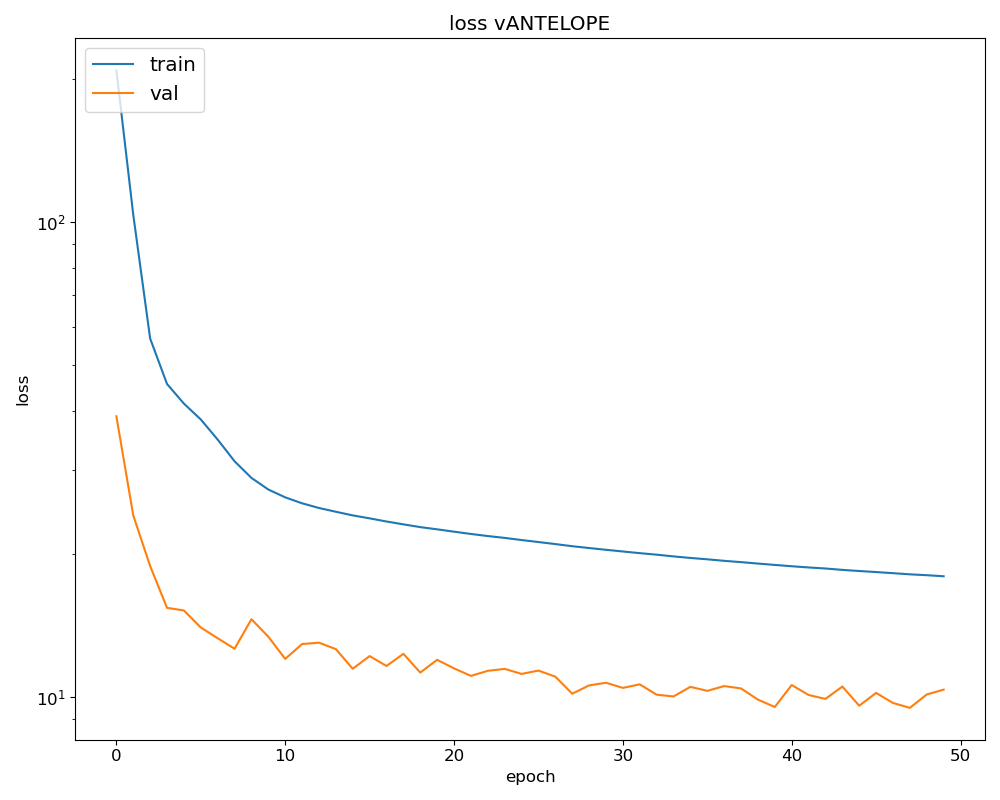
\includegraphics[width=0.5\textwidth]{figures/ml/antelope_loss}    
    \caption{ANTELOPE architecture loss during training as a function of epoch.
    \label{fig:antelope_loss}}
\end{figure}


%--------------------
\subsubsection{Performance}
\label{subsec:antelope_perf}

As with the PFN, the ANTELOPE performance is assessed via the area-under-curve (AUC) of the receiver operating characteristic (ROC) associated to evaluating the ANTELOPE on the test set of signal and background events.
Figure~\ref{fig:antelope_score} shows the output score distribution in data and total background MC, showing a very flat ratio and motivating the use of MC for studies of the ANTELOPE score.

\begin{figure}[!htbp]
\centering
   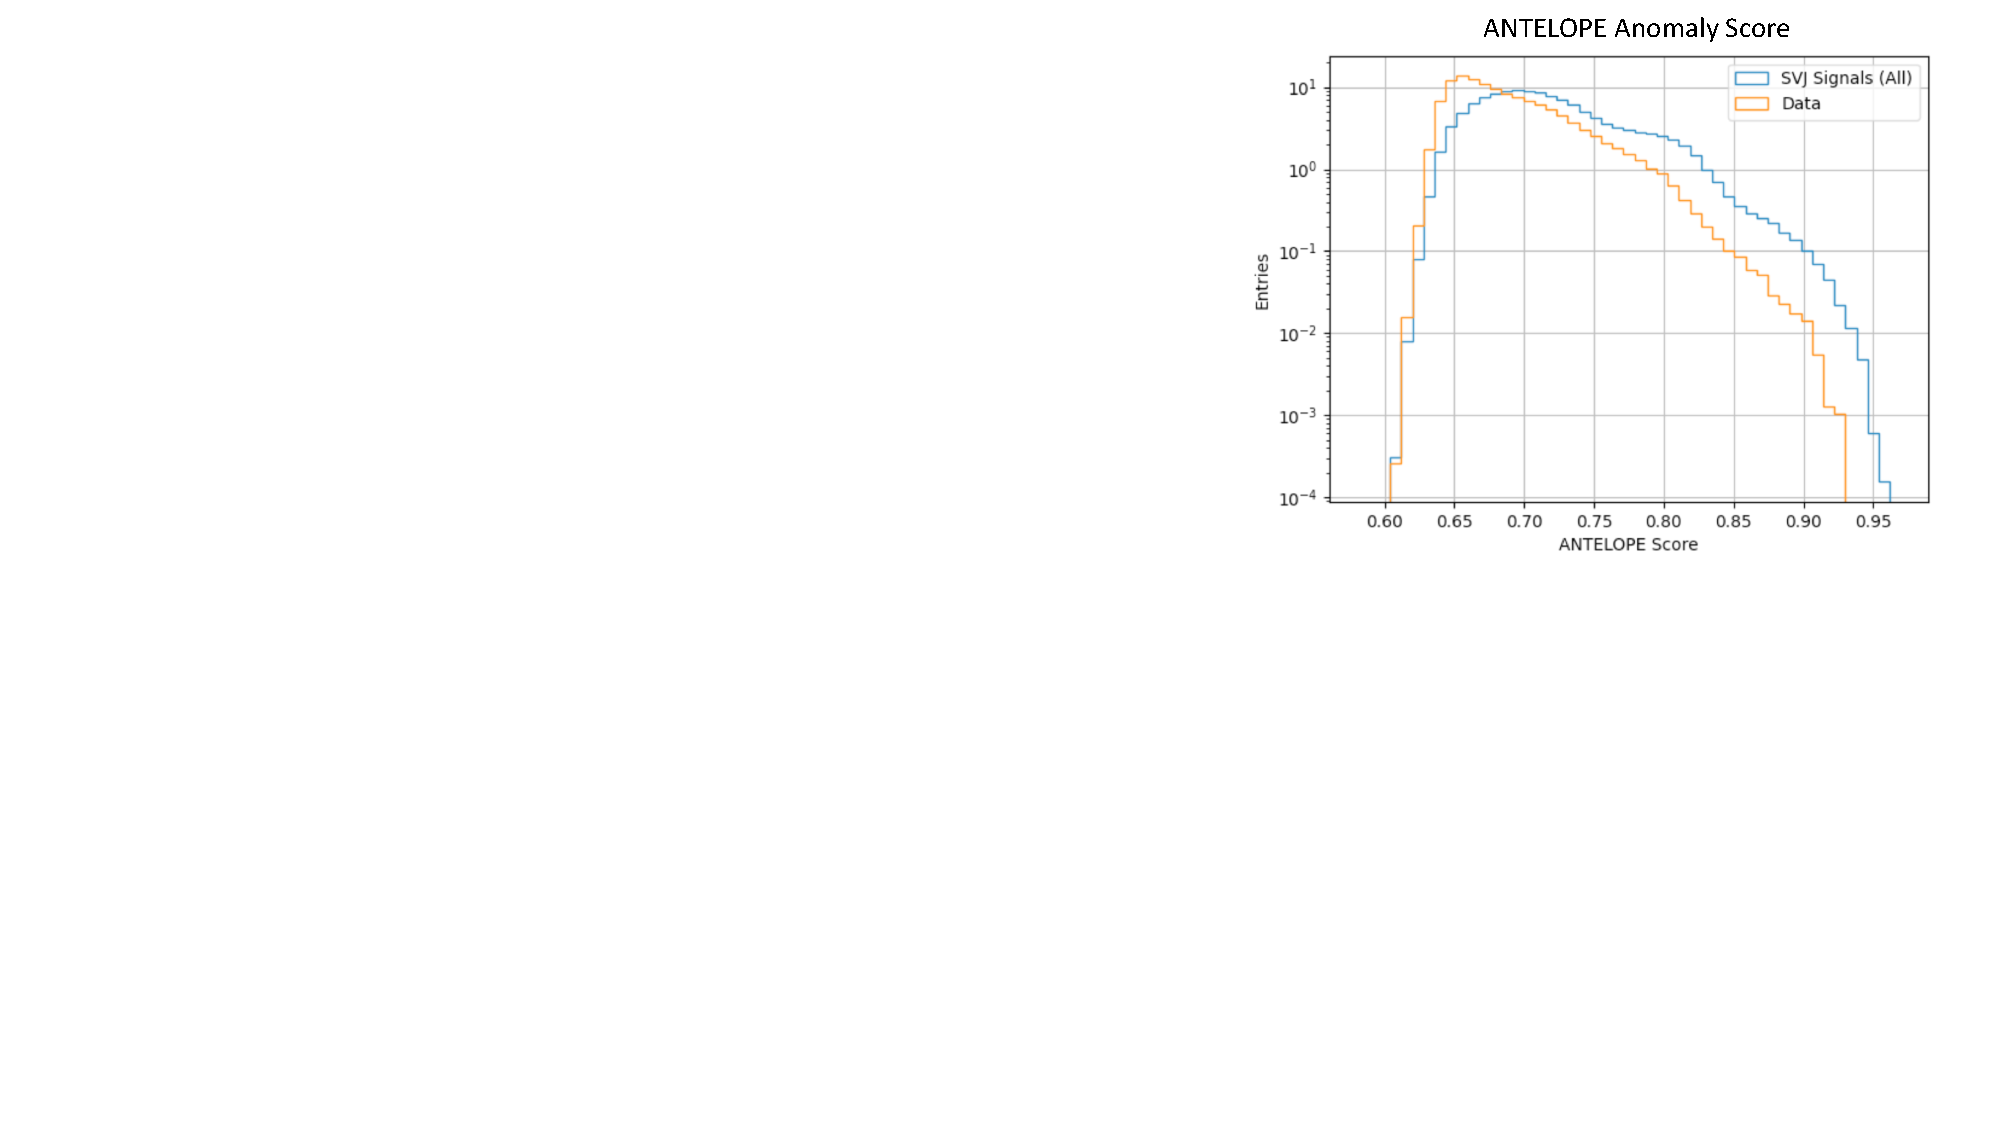
\includegraphics[width=0.48\textwidth]{figures/ml/antelope_score.pdf}
   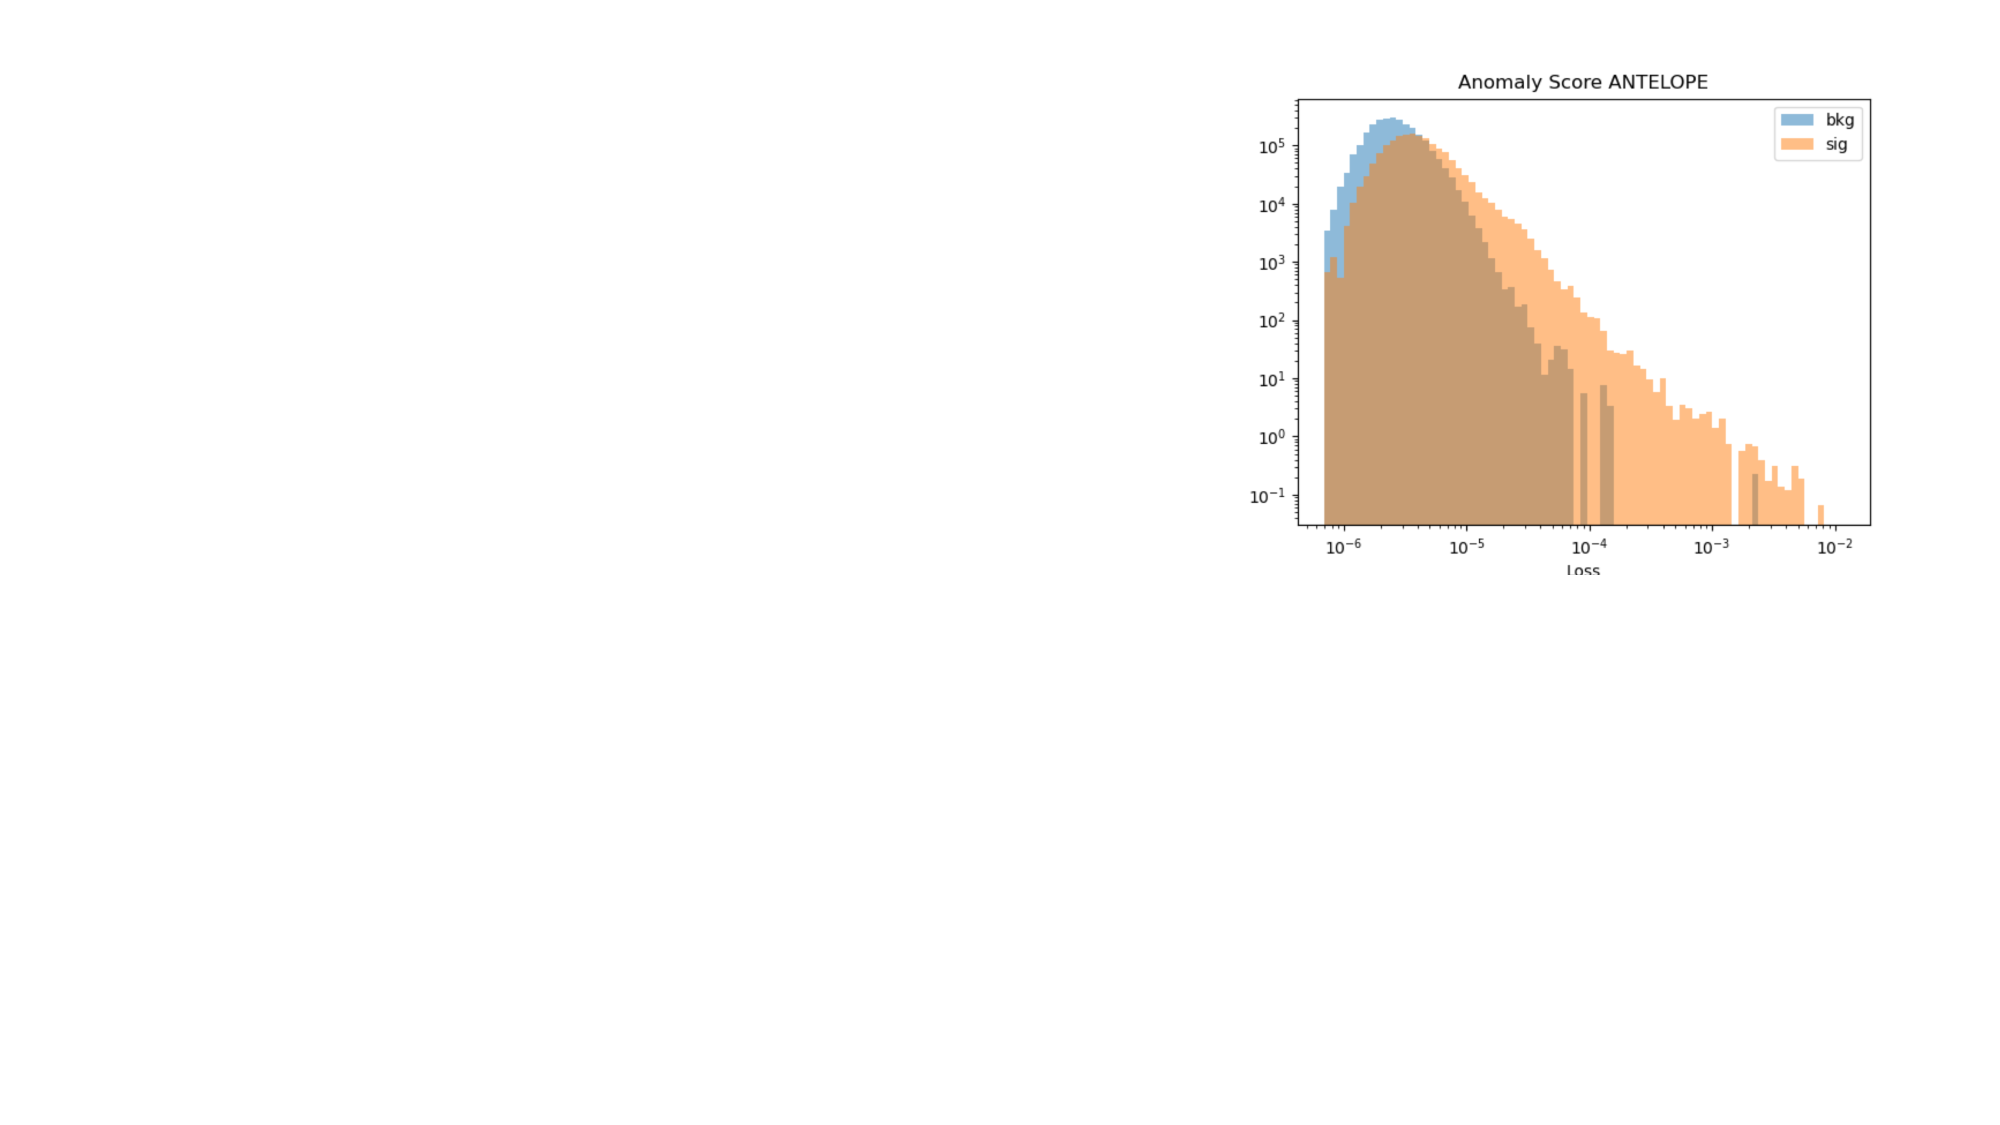
\includegraphics[width=0.48\textwidth]{figures/ml/antelope_score_mcsig}
    \caption{ANTELOPE score distribution comparing data and the total background MC (left), with good agreement observed between data and simulated background, and comparing all background MC to signals (right), revealing good discrimination power.
    \label{fig:antelope_score}}
\end{figure}

Figure~\ref{fig:antelope_AUC_score_grid} shows the AUC of the ANTELOPE across the SVJ signal grid, demonstrating strong discrimination capability even in the varying corners of phase space. 
Compared to the supervised PFN method, the ANTELOPE is not as performant (as expected due to the absence of signal model in training).
However, a selection on events with high ANTELOPE score nonetheless provides a 10-40\% increase in signal significance by removing background and isolating the long tail of anomalous events.

\begin{figure}[!htbp]
\centering
   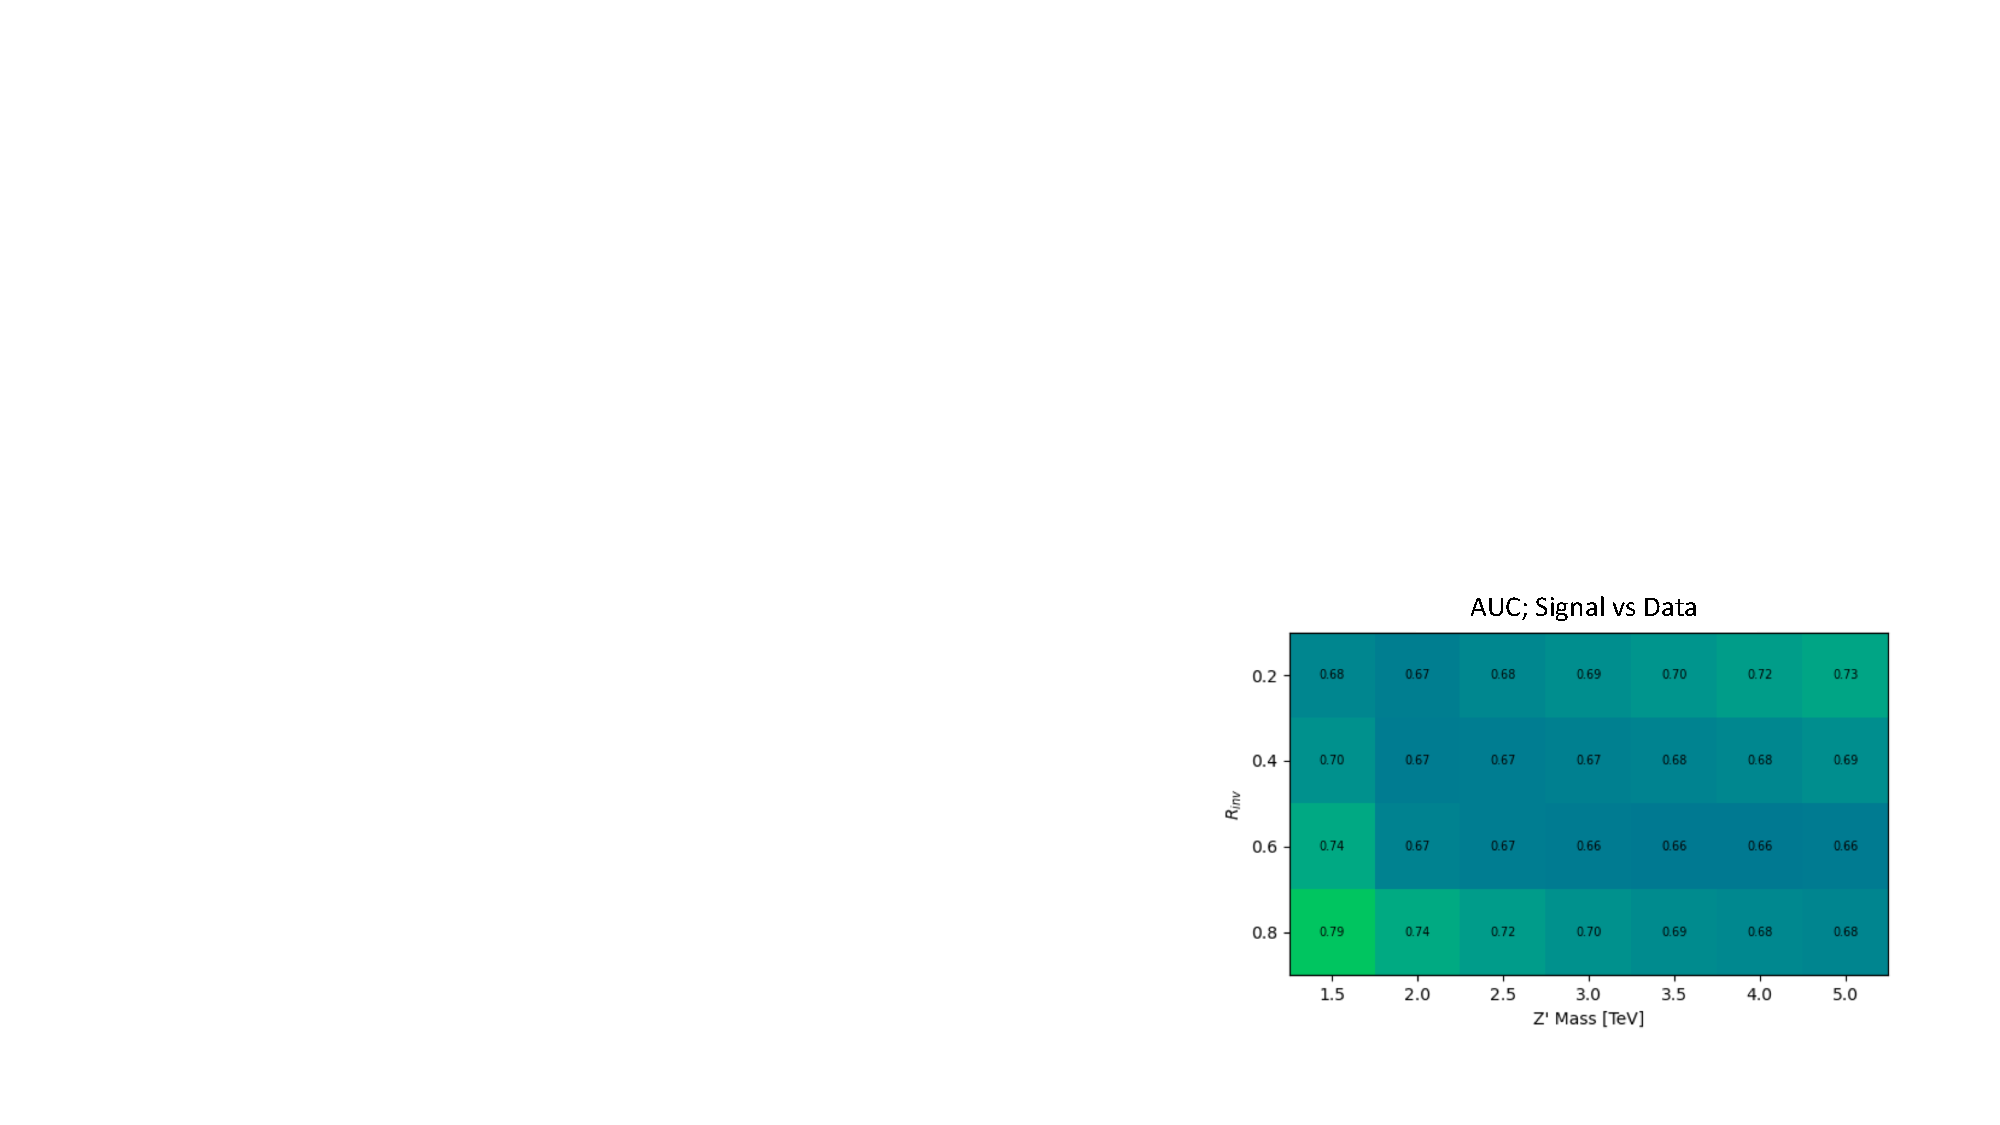
\includegraphics[width=0.7\textwidth]{figures/ml/antelope_AUC_score_grid}
    \caption{AUC from the ANTELOPE score for each signal in the SVJ grid.
    \label{fig:antelope_AUC_score_grid}}
\end{figure}

\paragraph{Model Independence} 

The unsupervised component of training the ANTELOPE network is expected to give it a more generalized sensitivity to new physics with \met~and jet activity, beyond the scope of the SVJ grid. 
To assess this, alternative signal models are evaluated with the trained ANTELOPE network, as optimized for the SVJ grid, and their sensitivity in the analysis selection is evaluated.

The following alternate signal models were considered: 
\begin{itemize}
\item Z' $\rightarrow$ $t\bar{t}$ 
\item W' $\rightarrow$ WZ 
\item Gluino pair production $\rightarrow$ R-hadron + LSP (\met) with gluino masses 2000/3000 GeV, LSP mass 100 GeV, and lifetime 0.03 ns (LSP = \textit{lightest supersymmetric particle})
\item Emerging jets s-channel with mass 1000 GeV and lifetime 1ns 
\end{itemize}

Figure~\ref{fig:antelope_altsig} shows the distribution of these signals in the PFN score and the ANTELOPE score.
This comparison reveals that ANTELOPE is sensitive to \met~in the event; it classifies signals with no real \met~, like the all-hadronic Z' and W' decays (given our imposed lepton veto) as data-like, but the distributions for signals with \met~such as SVJs, R-hadrons, and emerging jets have distributions with higher anomaly score tails.
\begin{figure}[!htbp]
\centering
   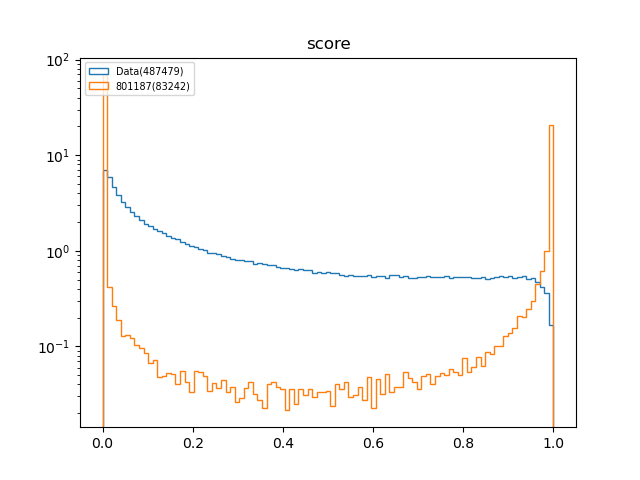
\includegraphics[width=0.48\textwidth]{figures/ml/pfn_altsignals}
   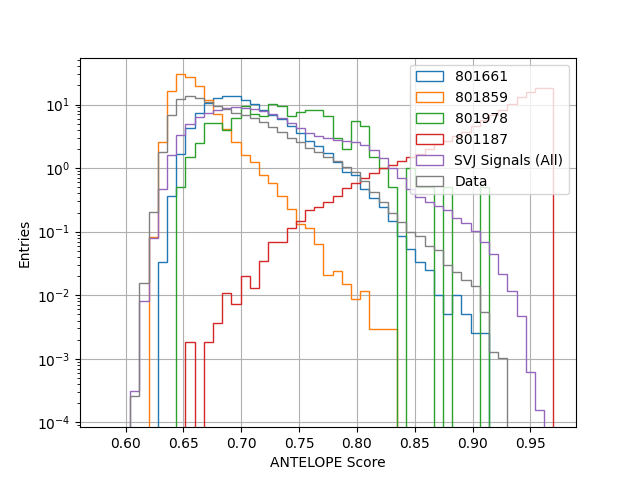
\includegraphics[width=0.48\textwidth]{figures/ml/antelope_altsignals}
    \caption{Comparing data and the alternate signal models for the PFN score (left) and ANTELOPE score (right). The emerging jet signal is an example of the gain of the model-independent ANTELOPE approach, where it has a bimodal shape in PFN score but is clearly tagged as anomalous by ANTELOPE.
    \label{fig:antelope_altsig}}
\end{figure}

Figure~\ref{fig:antelope_pfn_comp} shows a comparison of the sensitivity of the PFN and ANTELOPE regions across a variety of signals, including the combined SVJ signal used to train the PFN.
The benefit of the unsupervised stage of ANTELOPE in enhancing model independence is clearly seen through the boost in performance for other signal models, namely the gluino and emerging jet signals, which have more \met~than the W' and Z' signals (all-hadronic) that were also tested. 
As commented above, the PFN outperforms ANTELOPE as expected, because it was designed explicitly for the task of classifying SVJs from background, demonstrating the power of supervised learning for the model-specific approach.

\begin{figure}[!htbp]
\centering
   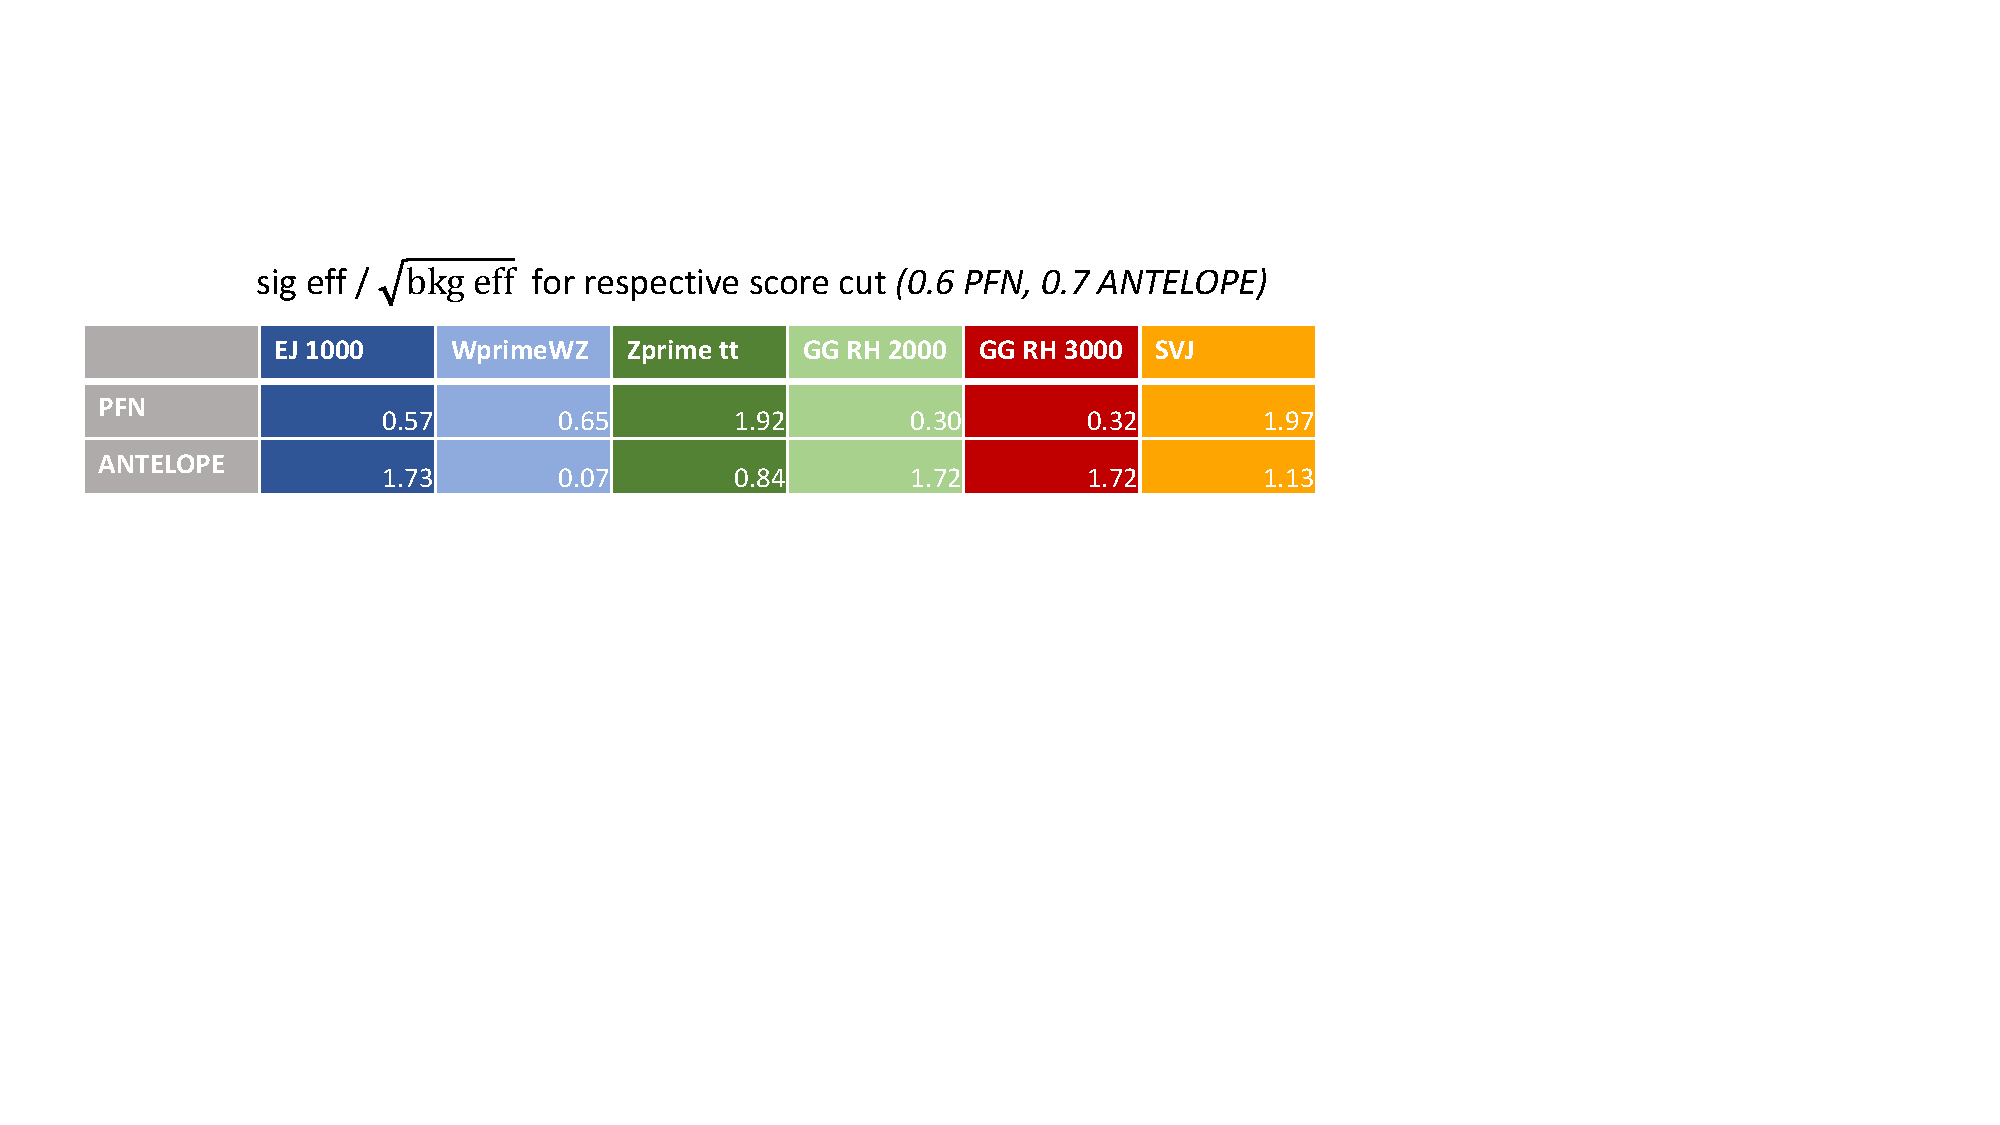
\includegraphics[width=0.95\textwidth]{figures/ml/antelope_pfn_comp}
    \caption{Comparing data and the alternate signal models in terms of sensitivity (S/$\sqrt{B}$) for the PFN and ANTELOPE tools, applying the selection that is used in the analysis. The ANTELOPE network is found to provide significant added sensitivity to alternate signals such as the gluino$\rightarrow$ R-hadron and emerging jets, which have higher \met~than the SVJs.
    \label{fig:antelope_pfn_comp}}
\end{figure}


Studies on the ANTELOPE architecture and comparisons to other methods can be found in Appendix~\ref{app:aevsantelope}.





